%!TEX root = ../greb.tex
% Тип документа
\documentclass[a4paper,12pt]{extarticle}

% Шрифты, кодировки, символьные таблицы, переносы
% \usepackage{cmap}
% \usepackage[T2A]{fontenc}
\usepackage[utf8]{inputenc}
\usepackage[russian]{babel}
% Это пакет -- хитрый пакет, он нужен но не нужен
\usepackage[mode=buildnew]{standalone}

\usepackage
	{
		% Дополнения Американского математического общества (AMS)
		amssymb,
		amsfonts,
		amsmath,
		amsthm,
		% Пакет для физических текстов
		physics,
		% misccorr,
		% 
		% Графики и рисунки
		wrapfig,
		graphicx,
		subcaption,
		float,
		tikz,
		tikz-3dplot,
		caption,
		csvsimple,
		color,
		booktabs,
		geometry,
		% 
		% Таблицы, списки
		makecell,
		multirow,
		indentfirst,
		%
		% Интегралы и прочие обозначения
		ulem,
		esint,
		esdiff,
		% 
		% Колонтитулы
		fancyhdr,
	} 
    
\usepackage{mathtools}
\mathtoolsset{showonlyrefs=true} 
\usepackage{pgfplots,pgfplotstable,booktabs,colortbl}
\usepackage{xcolor}
\usepackage{hyperref}
\usepackage{pythontex}
 % Цвета для гиперссылок
\definecolor{linkcolor}{HTML}{000000} % цвет ссылок
\definecolor{urlcolor}{HTML}{799B03} % цвет гиперссылок
 
\hypersetup{pdfstartview=FitH,linkcolor=linkcolor,urlcolor=urlcolor, colorlinks=true}
\hypersetup{pageanchor=false}
% Увеличенный межстрочный интервал, французские пробелы
\linespread{1.3} 
\frenchspacing 

\newcommand{\mean}[1]{\langle#1\rangle}

\begin{pycode}
##
def frexp10(decimal):
	parts = ('%e' % decimal).split('e')
	return float(parts[0]), int(parts[1])
##
\end{pycode}



% Функция для тех, кто использует pythontex. Представляет любое вещественное число в стандартном виде.
\newcommand{\frexp}[1]{
		\pyc{#10=frexp10(#1)} 
			\py{ round(#10[0],2)} 
				\cdot 10^{\py{#10[1]}} }

% const прямым шрифтом
\newcommand\ct[1]{\text{\rmfamily\upshape #1}}
\newcommand*{\const}{\ct{const}}
\usepackage{array}
\usepackage{pstool}

\geometry		
	{
		left			=	2cm,
		right 			=	2cm,
		top 			=	2.5cm,
		bottom 			=	2.5cm,
		bindingoffset	=	0cm
	}

%%%%%%%%%%%%%%%%%%%%%%%%%%%%%%%%%%%%%%%%%%%%%%%%%%%%%%%%%%%%%%%%%%%%%%%%%%%%%%%
	%применим колонтитул к стилю страницы
\pagestyle{fancy} 
	%очистим "шапку" страницы
% \fancyhead{} 
	%слева сверху на четных и справа на нечетных
\fancyhead[R]{}%\labauthors 
	%справа сверху на четных и слева на нечетных
% \fancyhead[L]{Отчёт по лабораторной работе №\labnumber}
\fancyhead[L]{\labtheme} 
	%очистим "подвал" страницы
% \fancyfoot{} 
	% номер страницы в нижнем колинтуле в центре
\fancyfoot[C]{\thepage} 

%%%%%%%%%%%%%%%%%%%%%%%%%%%%%%%%%%%%%%%%%%%%%%%%%%%%%%%%%%%%%%%%%%%%%%%%%%%%%%%

\renewcommand{\contentsname}{Оглавление}
\usepackage{tocloft}
\usepackage{secdot}
\sectiondot{subsection}


\begin{document}
\def\labauthors{Виноградов И.Д., Понур К.А., Шиков А.П.}
\def\labgroup{440}
\def\labnumber{1}
\def\labtheme{Исследование твердотельных структур методом ЭПР-спектроскопии}
\def\department{Кафедра квантовой радиофизики и электроники}
\begin{titlepage}

\begin{center}

{\small\textsc{Нижегородский государственный университет имени Н.\,И. Лобачевского}}
\vskip 1pt \hrule \vskip 3pt
{\small\textsc{Радиофизический факультет}}



\vfill
{\Large {\department}}

{\Large Отчет по лабораторной работе №\labnumber\vskip 12pt\bfseries \labtheme}
	
\end{center}

\vfill
	
\begin{flushright}
	{Выполнили студенты \labgroup\ группы\\ \labauthors}%\vskip 12pt Принял:\\ Менсов С.\,Н.}
\end{flushright}
	
\vfill
	
\begin{center}
	Нижний Новгород, \the\year
\end{center}

\end{titlepage}


\newpage
\section{Теоретическая часть}%


\section{Экспериментальная часть}%
\section{Исследование ЭПР в молекулах дифенила}%
\paragraph{Получение на экране осциллографа кривых поглощения и дисперсии сигнала ЭПР.}%
\label{par:1}
Для получения необходимой картины необходимо произвести следующие действия:
\begin{enumerate}
    \item Вставить образец в резонатор.
    \item Включить ВЧ-генератор и прогреть его в течение 5-ти минут; включить модулирующее поле.
    \item Подключить к выходу детектора измеритель мощности и при полностью выведенном аттенюаторе ($\alpha = 0$ ) настроить клистронный генератор по частоте
        на центр одной из зон по максимуму мощности, контролируемой измерительным прибором. В эксперименте, для дифенила максимум частоты 
        пришелся на $\nu = 8.99$ ГГц.
    \item Ввести волноводный аттенюатор балансного плеча ($\alpha = 100 \% $) и настроить его в резонанс (соответствует минимуму сигнала на выходе детектора.)
    \item Подключить выход детектора с соблюдением полярности на вход с соблюдением полярности на вход усилителя.
    \item Включить источник постоянного тока и, меняя величину тока через катушки магнита (зависимость $H(I)$ на рис.\ref{fig:1}), вывести на резонансное значение поле $H$, определяя момент по появлению на экране осциллографа 
        пары сигналов, соответствующих резонансному переходу. 

    \item Вывести волноводный аттенюатор ($ \alpha = 0$ ) и, перемещая плунжер балансного плеча, получить кривые $\chi'$ и  $\chi''$. (рис. \ref{fig:2})
     Кривой $\chi'$ соответствует значение тока $I' = 159 $ мА,  а кривой $\chi''$ -- $I'' = 169$ мА, что эквивалентно полю в 3550 и 3750 Гс соответственно.
\end{enumerate}


\paragraph{Измерение ширины линий поглощения сигнала ЭПР в единицах поля.}%

\paragraph{Расчет ширины линии в единицах частоты.}

\paragraph{Определение числа парамагнитных частиц в образце.}%


\begin{figure}[h!]
    \centering
    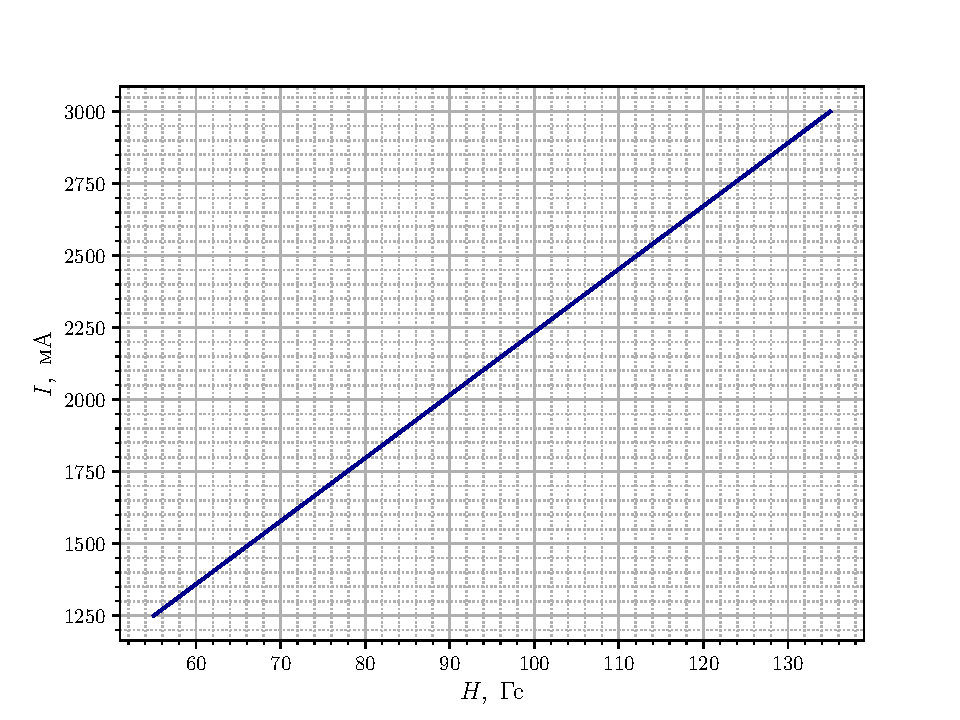
\includegraphics[scale=1]{fig/fig1}
    \caption{Градуировочный график зависимости магнитного поля $H$ от тока $I$}
    \label{fig:1}
\end{figure}

\begin{figure}[h!]
    \centering
    \includegraphics[scale=1]{example-image-a}
    \caption{Кривые $\chi'$ и  $\chi''$ на экране осциллографа}
    \label{fig:2}
\end{figure}


\end{document}
